\documentclass[12pt]{exam}
\usepackage[utf8]{inputenc}

\usepackage[margin=1in]{geometry}
\usepackage{amsmath,amssymb}
\usepackage{multicol}
\usepackage{mathrsfs}
\usepackage{graphicx}
\usepackage{multicol}
\usepackage[shortlabels]{enumitem}
\usepackage{scrextend}
\usepackage{xcolor}
\usepackage[normalem]{ulem}
\usepackage{optprog}

\newcommand{\class}{SA405, Fall 2020}
\newcommand{\term}{}
\newcommand{\examnum}{Exam 2}
\newcommand{\examdate}{6 November 2020}
\newcommand{\timelimit}{50 Minutes}

\pagestyle{head}
\firstpageheader{}{}{}
\runningheader{\class}{\examnum\ - Page \thepage\ of \numpages}{\examdate}
\runningheadrule

%% Answer box macros
%% \answerbox{alignment}{width}{height}
\newcommand{\answerbox}[3]{%
  \fbox{%
    \begin{minipage}[#1]{#2}
      \hfill\vspace{#3}
    \end{minipage}
  }
}

%% \answerboxfull{alignment}{height}
\newcommand{\answerboxfull}[2]{%
  \answerbox{#1}{6.38in}{#2}
}

%% \answerboxone{alignment}{height} -- for first-level bullet
\newcommand{\answerboxone}[2]{%
  \answerbox{#1}{6.0in}{#2}
}

%% special boxes
\newcommand{\wordbox}{\answerbox{c}{1.2in}{.7cm}}
\newcommand{\catbox}{\answerbox{c}{.5in}{.7cm}}
\newcommand{\letterbox}{\answerbox{c}{.7cm}{.7cm}}

\printanswers
%\noprintanswers
\begin{document}

\noindent
\begin{tabular*}{\textwidth}{l @{\extracolsep{\fill}} r @{\extracolsep{6pt}} r}
\textbf{\class} &&\textbf{\examnum}\\
\textbf{\term} &&\textbf{\examdate}\\
 && \\
 && \\
\emph{Midshipmen are persons of integrity.}& \textbf{Name:} & \makebox[2.2in]{\hrulefill}\\\\
%\textbf{Time Limit: \timelimit} &  & \makebox[2in]{\hrulefill}
\end{tabular*}

\noindent
\rule[2ex]{\textwidth}{2pt}

%This exam contains \numpages\ pages (including this cover page) and \numquestions\ questions.\\
%Total of points is \numpoints.

\begin{itemize}
%\item You may pull the pages apart and then staple them together at the end.  I prefer not to see your name when I am grading, so only write your name on the first page (unless submitting pages unstapled).

\item No books, notes, or any other outside help % or calculators
% that do symbolic manipulation (such as TI-89 or TI-92)
 allowed. %{\bf One} 8.5 by 11 inch formula/note sheet is allowed.

%\item You may use your calculator on this test.

\item Show work clearly and neatly.

\item Define all notation used.
%\item If you need more space than is provided, use the back of the previous page.

\item Please read each question carefully.
If you are not sure what a question is
asking, ask for clarification.

\item If you start over on a problem, please CLEARLY indicate what your final
  answer is, along with its accompanying work.

%\item All formulations must have descriptions of any indices, parameters, and decision variables used. All constraints must be described.
\end{itemize}

\bigskip
\begin{center}
Grade Table (for teacher use only)\\
\addpoints
\gradetable[v][questions]
\end{center}

\noindent
\rule[2ex]{\textwidth}{2pt}

\newpage %%%%%%%
\begin{questions}
%\question  The goal of the famous graph coloring problem is to find the minimum number of colors required to color the vertices of a graph so that no two adjacent vertices have the same color.  For this single-color variation on graph coloring, we  want to color as many vertices ``red'' as possible, without coloring adjacent vertices.  Consider the graph below.  Let $x_i = 1$ if vertex $i$ is colored red, and 0 otherwise.

%\begin{center}
%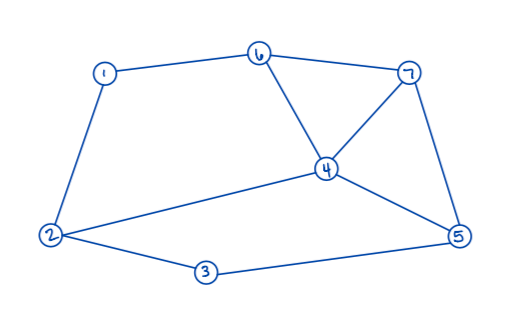
\includegraphics[width=0.5\textwidth]{graph1}
%\end{center}

%\begin{parts}
%\part Formulate a concrete objective function, as well as a set of concrete constraints that enforce the logic that at most one of any pair of adjacent vertices can be selected.  (For example, at most one of 4 and 6 can be selected.)
%\part Write the model in abstract form.  Define any sets that are required.  (You shouldn't need any parameters.)
%\end{parts}

\question
Answer the following

\begin{parts}
\part [14] You're modeling an integer program on continuous variables ($x_1$, $x_2$, and $x_3$). To complete the model, one of the following two constraints needs to be included:
\begin{optprog}
& 2x_1 + 3 x_2 - 3 x_3 & \geq 10 & \\
&  x_1 - x_2 + 2x_3 & \leq 30 & 
\end{optprog}
Use binary variable $y$ to modify above constraints in order to execute the following strategy; If $y=0$, the first constraint (constraint 1) is included, and if $y=1$, then second constraint (constraint 2) is included in the model.
\begin{solution}[2.5in]

\begin{optprog*}
& 2x_1 + 3 x_2 - 3 x_3 & \geq & 10-My & \\
&  x_1 - x_2 + 2x_3 & \leq & 30+M(1-y) &\\
\end{optprog*}
where $M$ represents a big number.
\end{solution}

\part Consider the subtour elimination constraints in the traveling salesperson problem on \textbf{7 total nodes}. Next to each of the following set sizes, circle yes or no to indicate whether you would eliminate subtours of that size (e.g., if you circle yes next to 3, this means you would want to eliminate all subtours on sets of size 3).
	\begin{subparts}
	\subpart[2] Sets of size 2? \vspace{2mm} YES or NO
	\begin{solution}
	No
	\end{solution}
	\subpart[2] Sets of size 3? \vspace{2mm} YES or NO
	\begin{solution}
	Yes
	\end{solution}
	\subpart[2] Sets of size 7? \vspace{2mm} YES or NO
	\begin{solution}
	No
	\end{solution}
	\end{subparts}


\part [10] Suppose you're modeling a vehicle routing problem with 2 vehicles on 8 nodes (specifically nodes 0, 1, 2, 3, 4, 5, 6, 7). Write the concrete constraints which tell the number of edges that must be connected to node 0 (the depot) and node 4.
\begin{solution}

For node 0, we would have:
\[
x_{0,1} + x_{0,2} + x_{0,3} + x_{0,4} + x_{0,5} + x_{0,6} + x_{0,7} = 2*2 = 4
\]

For node 4, we would have:
\[
x_{0,4} + x_{1,4} + x_{2,4} + x_{3,4} + x_{4,5} + x_{4,6} + x_{4,7} = 2
\]

\end{solution}

\end{parts}



\newpage
\question In order to improve food variety, you've decided, along with one of your friends, to open up two taco stands on the yard. You're trying to determine where to open these two stands. You've identified 4 possible locations for your stands: Nimitz, Gate 1, Chauvenet courtyard, and Bancroft. You want to service demand at each of the following buildings: Nimitz (NI), Visitor center (VC), Chauvenet (CH), Michelson (MI), Alumni Hall (AH), Bancroft (BA), and Ward (WA). The table below gives the distances between each potential taco stand location and each customer as well as the demand of each customer:

\begin{center}
\begin{tabular}{c|ccccccc}
\hline
                          & \multicolumn{7}{c}{Destinations}  \\
Potential Locations       &  NI & VC & CH & MI & AH & BA & WA \\ \hline
 Nimitz (NI)              &  0  & 20 & 8  & 7  & 3  & 11 & 15  \\
 Gate 1 (G1)              &  15 & 1  & 12 & 12 & 15 & 10 & 6   \\
 Chauvenet Courtyard (CC) &  6  & 15 & 1  & 1  & 8  & 5  & 12 \\
 Bancroft (BA)            &  11 & 10 & 5  & 5  & 12 & 0  & 7 \\ \hline
 Demand                   &  50 & 12 & 25 & 22 & 7  & 80 & 15 \\
\end{tabular}
\end{center}

A customer can only be serviced if its distance is at most 12 units away.

Consider the partial model given below:

\textbf{\underline{Sets}}

Let $S$ be the set of potential locations for your taco stand $S = \{NI, G1, CC, BA\}$ \\
Let $C$ be the set of customers of your taco stand $C = \{NI, VC, CH, MI, AH, BA, WA\}$\\

\textbf{\underline{Parameters}}

Let $h_c$ be the demand of customer $c$ for all $c \in C$ \\
Let $d_{s,c}$ be the distance between customer $c$ and taco stand $s$ for all $c \in C$ and for all $s \in S$\\
Let $N_c$ be the neighborhood of customer $c$ for all $c \in C$.

\textbf{\underline{Decision Variables}}

Let $x_s = 1$ if a taco stand is placed at location $s$ for all $s \in S$.

\begin{parts}
\part [5] A taco stand is in the neighborhood of a customer if it is at most 12 units away. What is $N_{NI}$ and $N_{WA}$?

\begin{solution}[2in]
The neighborhood of NI is all suppliers at most 12 units away. This means that:
\[
N_{NI} = \{ NI, CC, BA\}
\]

Likewise, the neighborhood of WA is all suppliers at most 12 units away. Thus:
\[
N_{WA} = \{ G1, CC, BA \}
\]
\end{solution}

\part Since you only have 2 taco stands, you decide to formulate an IP to optimally determine where to place your taco stands. The goal of this IP is to cover as much demand as possible with the limitation that only two taco stands can open.
	\begin{subparts}
	\subpart [5] Introduce any new decision variables needed to formulate this IP. If none are needed write NONE NEEDED and continue to question ii
	\begin{solution}[1.15in]
	We need to define a new variable here $y_c$ which equals 1 if customer $c$ is covered and $y_c = 0$ if customer $c$ is not covered for all $c \in C$
	\end{solution}
	\subpart [5] Write a concrete constraint which says that exactly 2 taco stands can be opened.
	\begin{solution}[1.15in]
	\[
	x_{NI} + x_{G1} + x_{CC} + x_{BA} = 2
	\]
	\end{solution}
	\subpart [10] Write an objective function which maximizes the total demand covered.
	\begin{solution}[1.15in]
	\[
	\text{maximize: } \sum_{c \in C} h_c y_c
	\]
	\end{solution}
	\subpart [10] In order to formulate this correctly, each customer node must either be covered or not covered. Write a concrete constraint for Alumni Hall that says if no taco stand is opened in its neighborhood, then it is not covered. Once you have written this constraint, explain its logic in words (it is suffice to say if BLEH then BLAH else MEH).
	\begin{solution}[2in]
	We need to write a constraint that says $y_{AH}$ can only be covered if one of the nodes in its neighborhood is selected. First, we consider it's neighborhood which is $N_{AH} = \{NI, CC, BA \}$. So my constraint I want is:
	\[
	x_{NI} + x_{CC} + x_{BA} \geq y_{AH}
	\]
	
	The logic of this constraint is as follows. If we place the taco stand at either NI, CC, or BA, it covers AH. Thus, $y_{AH}$ will become $1$. Conversely, if none of these facilities are built, then $x_{NI} = x_{CC} = x_{BA} = 0$ thereby forcing $y_{AH}$ to be 0 since it will not be covered.	
	
	\end{solution}
	\end{subparts}
	\newpage
%\part Continuing this question, suppose that each of your taco stands has a capacity of 100 tacos. Suppose we define a new variable $z_{s,c}$ which equals 1 if \textbf{all} of the demand of customer $c$ is covered by taco stand $s$. (Note that this means that each customer location can only be served by a single taco stand).
%	\begin{subparts}
%	\subpart [5] For the taco stand at Nimitz, write a concrete constraint which enforces that it can only be assigned customers so that the demand does not exceed 100 tacos. \emph{Hint: Consider what customers can be serviced by NI and you only need to use the $z_{s,c}$ variables}.
%		\begin{solution}[2.5in]
%	First, let's determine which customers can be serviced by NI. A customer can be serviced by NI if its 12 units or less away in distance. Thus, the set of customers that can be serviced by NI are: $\{NI, CH, MI, AH, BA\}$. So my final constraint would be:
%	\[
%	50 z_{NI, NI} + 25 z_{NI, CH} + 22 z_{NI, MI} + 7 z_{NI, AH} +80 z_{NI, BA}  \leq 100
%	\]
%	\end{solution}
%	\subpart [5] Convert your constraint above to an abstract form for each supply node $s \in S$. \emph{Hint: You can define a new parameter/set if you would like, but you can write this constraint using only the notation defined so far.}
%	\begin{solution}[1.5in]
%	I need one of these constraints for each $s \in S$. I get this with the following constraint:
%	\[
%	\sum_{c: s \in N_c} h_c z_{s,c} \leq 100 \text{\hspace{1mm} For all $s \in S$}
%	\]
%	\end{solution}
%	\end{subparts}
\end{parts}


\newpage 

\question The Military Command Center 'East'  needs to install special secure communication lines between the Command Center (CC) and five of Military Installation posts (MI1,..., MI5) under its command. The  communication line from a  MI post need not be connected directly to the  CC. It can be connected indirectly by being connected to another MI post that is connected (directly or indirectly) to the CC. The only requirement is that every MI post  be connected by some route to the CC.
The  installation of a special communication line is  costly; it costs $100,000$   per  mile. Hence, the total cost of installation of special communication lines is $100,000$ times the number of miles involved, where the distances (in miles) between CC and MIs and between MIs  are  given in the table below:

\begin{center}
\begin{tabular}{c|cccccc}
\hline
                         & \multicolumn{6}{c}{Distances in miles}  \\
                         &  CC       & MI1  & MI2  & MI3  & MI4  & MI5  \\ \hline
Command center (CC)      &  -        & 190  & 70   & 115  & 270  & 160   \\
 MI1                     &           & -    & 100  & 110  & 215  & 50    \\
 MI2                     &           &      & -    & 140  & 120  & 220    \\
 MI3                     &           &      &      & -    & 175  & 80   \\ 
 MI4                     &           &      &      &      & -    & 310  \\
 MI5                     &           &      &      &      &      & -  \\ \hline
\end{tabular}
\end{center}

The CC wants to determine which pairs of MIs, and CC and MIs should be
directly connected by special  communication lines in order to connect every
MI (directly or indirectly) to the CC at a minimum total cost.

Below we list the sets, parameters and variables of the  model

\textbf{\underline{Sets}}

Let $S$ be the set the CC and MIs $S = \{CC, MI1, MI2, MI3, MI4, MI5 \}$ \\
Let $E$ be the set of edges $E = \{(i,j) : i, j \in S, i< j\}$ \\

\textbf{\underline{Parameters}}

Let $d_{i,j}$ be the distance between nodes $i$  and $j$ for all  $i, j \in S$ in miles. \\

Let $P$ be the the price per mile of the special communication line.

\textbf{\underline{Decision Variables}}

Let $x_{i,j} = 1$ if a communication line is laid between nodes $i$  and $j$ for all  $i, j \in S$.


\begin{parts}
\part [2] Which type of Network optimization model best describes this problem?
\begin{solution}[0.5in]

Minimum Spanning Tree Model
\end{solution}

\part [5]  Write the objective function for the concrete model. You can use ellipses, however, write at least 3 terms explicitly.
\begin{solution}

\begin{optprog*}
Minimize & 190x_{CC,MI1}+70x_{CC,MI1}+ \cdots + 310x_{MI4,MI5}
\end{optprog*}
\end{solution}

\newpage

\part [8] Write  a concrete  constraint  that ensures a given node is  part of at least one edge for each of the following nodes: CC, MI1, and MI5. 
\begin{solution}[2in]
\begin{optprog*}
Node CC: & x_{CC,MI1}+x_{CC,MI2}+ \cdots + x_{CC,MI5} & \geq 1 \\
Node MI1: & x_{CC,MI1}+x_{MI1,MI2}+ \cdots + x_{MI1,MI5} & \geq 1 \\
Node MI 5: & x_{CC,MI5}+x_{MI1,MI5}+ \cdots + x_{MI4,MI5} & \geq 1 \\
\end{optprog*}
We have 6 such constraints, for each node one.
\end{solution}

\part [5] How many edges must the optimal solution have?  Write the concrete constraint that ensures the solution has exactly that many edges. 

\begin{solution}[1in]
Since we have 6 nodes,  the  MST will have $6-1=5$ edges.
	\[
		\sum_{(i,j) \in E} x_{i,j} =5
	\]
\end{solution}



\part Suppose that at one stage of  solving the problem the following solution is obtained: 

$(CC,MI2), (CC,MI5), (MI1,MI5), (MI1,MI2), (MI2,MI3), (MI3,MI4)$

	\begin{subparts}
		\subpart [3] Graph this solution. 
			\vspace{2in}
			\begin{solution}
	
			\end{solution}
		\subpart [2] Is this  solution feasible? Answer Yes or No.
		\begin{solution}[0.5in]
			NO
			\end{solution}
		\subpart [10] If Yes, explain. If Not,  write the constraint that will prevent this solution from occurring again.
		\begin{solution}
This solution has a cycle $$(CC,MI2), (CC,MI5), (MI1,MI5), (MI1,MI2).$$ MST cannot have cycles, hence, they need to be eliminated. The set of nodes in the cycle is $S=\{CC, MI1, MI2, MI5\}$, therefore, the concrete cycle elimination constraint is
\[
 x_{CC,MI1}+x_{CC,MI2}+ x_{CC,MI5}+ x_{MI1,MI2}+ x_{MI1,MI5}+ x_{MI2,MI5}  \leq  4-1 =3
\]
			\end{solution}
	\end{subparts}
\end{parts}

\newpage


\end{questions}
\end{document}

